\documentclass{article}
\usepackage{amsmath, graphicx, amsfonts, caption, subfig, keyval, algorithm, algorithmic}
\usepackage{xcolor}
\usepackage{hyperref}
\captionsetup{justification=centering}
\newcommand{\R}{\mathbb{R}}
\newcommand{\C}{\mathcal{C}}
\newcommand{\X}{\mathcal{X}}
\DeclareMathOperator*{\argmin}{\arg\!\min}

\begin{document}
\title{AM221 Final Project Proposal}
\author{Taylor Killian \& Leonhard Spiegelberg}
\maketitle

\begin{abstract}
To be filled with an interesting summary of our work and results

\end{abstract}

%% Leos thoughts

\section{Dictionary Learning as 2-stage supermodular minimzation}
The introduced problem of Dictionary learning, which in its general form can be seen as
\[
\min_{D, R, \theta, \lambda} f(D, R, X) + g(D, \theta) + h(R, \lambda)
\]
where $f$ describes the objective function used to measure goodness of approximation of $X$ through $D, R$, $g$ describing suitable constraints on the dictionary, $h$ on the representation respectively.
With an input dataset $X=[x_1, \dots, x_k],  x_i \in \R^d,  X \in \R^{d\times k}$ we wish to find a dictionary $D \in \R^{d\times n},  \mathcal{D} = [d_1, \dots, d_n]$ and a representation $\mathcal{R}=[r_1,\dots,r_k], \ r_i\in\R^n, \ \mathcal{R}\in\R^{n\times k}$, such that both $\|X-\mathcal{D}\mathcal{R}\|_F^2$ is minimized and the representations $r_i$ are "sparse enough". To limit the dictionary becoming infinitely large (or small) we introduce a constraint on the dictionary's columns. For this any sufficient norm can be used. An often used norm is the $l_2$-norm. 
Thus for the dictionary learning problem we introduce the problem with constraints
\begin{alignat}{5}
         &\min_{D, R} \|X \ -D R\|_F^2  & \quad   \\
         &\text{s.t.}  \quad  &\|d_j\|_2 \leq 1&, \forall j=1, ...,n  \quad \\
         &  \quad  &\|r_i\|_0 \leq t&, \forall i=1, ...,k  \quad 
\end{alignat}

\textcolor{red}{Description of constraints here}


Using Lagrange multipliers this can be brought to the general form above
\[
\min_{D, R, \theta, \lambda} \|X \ -D R\|_F^2 + \sum_{j=1}^m \theta_j (\| d_j\|_2 - 1)+ \sum_{i=1}^k \lambda_i (\| r_i \|_0 - t)
\]
I.e. the functions are
\[
\begin{split}
f(D, R, X) &:= \|X \ -D R\|_F^2 \\
g(D, \theta) &:= \sum_{j=1}^n \theta_j (\| d_j\|_2 - 1) \\
h(R, \lambda) &:= \sum_{i=1}^k \lambda_i (\| r_i \|_0 - t)
\end{split}
\]
\textcolor{red}{How to bring this to the penalty function form?}

The difficulty in solving this problem comes from the mathematical challenge the $\| . \|_0$ norm yields. To understand this better confer \autoref{fig:l012plot}.
\begin{figure}
\centering
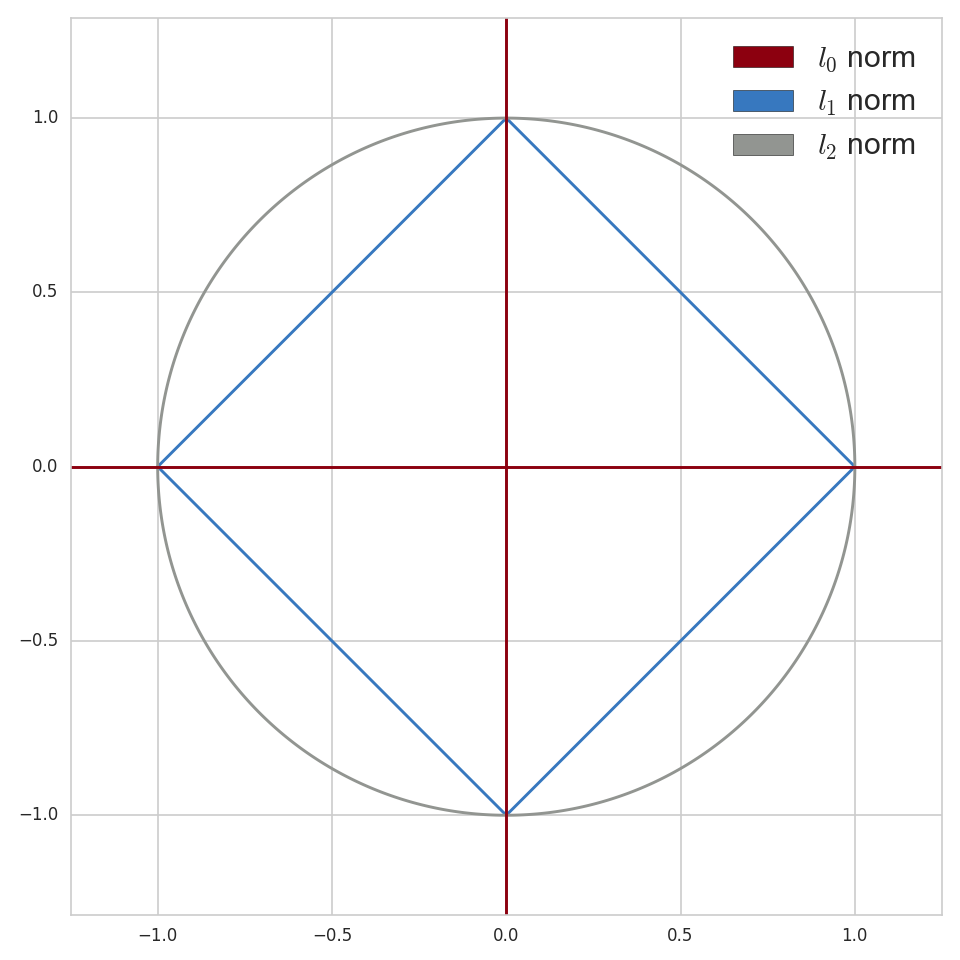
\includegraphics[scale=0.3]{img/l012_norms.png}
\caption{contour plot of the $l_0, l_1, l_2$ norm at levelset $L_1(f) := \lbrace x \in \R^2 : f(x) = 1 \rbrace $. Note that for any space $\R^d$, the image of the $l_0$ consists of $d+1$ values ($\lbrace 0, ..., d \rbrace $).}
\label{fig:l012plot}
\end{figure}
Let $x \in \R^d$
\[
l_0(x) := (\#i : x_i \not= 0)
\]
\textcolor{red}{here describe different norms...}
the goal is to find a norm that sort of converges to the infinite + of the l0 norm
\\

\textcolor{red}{Put here section about possible relaxations of l0 norm (related literature)}

\subsubsection{Two stage thoughts}
We will now relax the problem by formulating it into two stages:
\begin{enumerate}
\item solve for fixed $D, \theta$ the minimization to obtain optimal $R, \lambda$.
\item solve optimization for $D, \theta$ with obtained values
\item repeat previous steps until done
\end{enumerate}
\textcolor{red}{This is actually the method of optimal directions!}
In the traditional method of optimal directions (\textcolor{red}{ref here}) the subproblem $\min_{R, \lambda} f(D, R, X) + g(D, \theta) + h(R, \lambda)$ is solved either by various relaxation methods (i.e. LASSO, Matching Pursuit(\textcolor{red}{maybe describe here})), however for our approach we want to embedd the problem into a combinatorial optimization framework, which guarantees us bounds on optimality. Recent work done by \cite{weaklyalpha} showed that the subproblem of finding an optimal representation with a given dictionary is equivalent to Sparse Multiple Linear Regression (SMLR) and can be reformulated as a $\alpha$-weakly supermodular function. We will now show how to obtain this formulation:
Remember
\[
\begin{split}
\min_{R, \lambda} f(D, R, X) + g(D, \theta) + h(R, \lambda) \\
= \min_{R, \lambda} \|X -D R\|_F^2 + \sum_{j=1}^n \theta_j (\| d_j\|_2 - 1)+ \sum_{i=1}^k \lambda_i (\| r_i \|_0 - t)
\end{split}
\]
then let $S \subseteq [n]$ be a set of column indices for the dictionary. From now onwards we will assume that the given, fixed dictionary is normalized, i.e. $\forall d_i: \|d_i \|_2 = 1$. This allows us to remove the term $g(D, \theta)$. Define now $D_S$ as the matrix obtained from $D$ with all columns not indexed by $S$ to be set to zero. $D_S^+$ is the pseudoinverse which can be obtained i.e. via singular value decomposition when $D_S = U\Sigma V^T$ through $D_S^+ = V \Sigma^+ U^T$.
Then the problem can be equivalently stated as
\[
\begin{split}
 \min_{R, \lambda} \|X  -D R\|_F^2 + \sum_{i=1}^k \lambda_i (\| r_i \|_0 - t)\\
 \Longleftrightarrow 
  \min_{S \subseteq [n], |S| \leq t} \|X  -D_SD_S^+ X\|_F^2
 \end{split}
\]
\cite{weaklyalpha} have shown that the objective function $f(S) := \|X  -D_SD_S^+ X\|_F^2$ of this optimization problem is $\alpha$-weakly supermodular with 
\[ 
\alpha = \max_{\tilde{S} \subseteq [n]}\| D_{\tilde{S}}^+ \|_F^2
\]

\subsection{How to combine it}
...
\section{Introduction} \label{introduction}
Introduce the problem and it's complexities

\section{Background Information} \label{background}
\subsection{Background}
Here we'll want to add some information about Sparse regression, set functions and definitions of sub modular and super modular, Dictionary Selection, Greedy Methods, etc.

\subsection{Related Work}
A simple overview of prior work


\section{Methods} \label{methods}

Place holder section to begin to outline our work

\begin{algorithm}
  \caption{Notional algorithm}
  \label{alg:compass}
\begin{algorithmic}
  \STATE  Figure out optimal arrangement of rows and columns of input data
  \WHILE{there's still time in the semester}
  \IF{$f(p_k + s_k\lambda_i) < f(p_k)$ for some $\lambda_i$}
  \STATE $p_{k+1} = p_k + s_k\lambda_i$
  \STATE $s_{k+1} = s_k$
  \ELSE
  \STATE $p_{k+1} = p_{k}$
  \STATE $s_{k+1} = \alpha s_k$
  \ENDIF
  \ENDWHILE
  \RETURN VICTORIOUS
\end{algorithmic}
\end{algorithm}

\section{Experiments} \label{experiments}

Hold for applying our methods

\subsection{Results} \label{results}

The results of our algorithms against others

\section{Conclusions \& Future Work}
\subsection{Conclusions}
We will have done it!
 
\subsection{Future Work}
Rule the world 

\bibliographystyle{plain}
\bibliography{bibliography}

\end{document}